\documentclass[12pt, titlepage]{article}
\usepackage[utf8]{inputenc}
\usepackage[ngerman]{babel}
\usepackage{graphicx}
\usepackage[a4paper,width=150mm,top=25mm,bottom=25mm,bindingoffset=6mm]{geometry}
\usepackage{amsmath}
\usepackage{amssymb}
\usepackage[table,xcdraw]{xcolor}
\usepackage[nopostdot,toc,acronym,nomain,nonumberlist]{glossaries}
\usepackage[rightcaption]{sidecap}
\usepackage[export]{adjustbox}
\usepackage{eurosym}
\usepackage{tabularx}
\usepackage{multirow}
\usepackage{caption}
\usepackage{fancyhdr}
\usepackage{float}
\pagestyle{fancy}
\fancyhead{}
\fancyfoot{}
\fancyfoot[R]{\thepage}
\setlength{\headheight}{14.5pt}
\usepackage{csquotes}
\usepackage{biblatex}
\usepackage{csvsimple}
\usepackage{subcaption}
\usepackage{hyperref}

\addbibresource{Bibliographie.bib}

\title{\textbf{Bericht zum Seminar:\\[1cm]Praktische Analyse räumlicher Daten \\in R (Sommersemester 2019)}}

\author{\textbf{Betreuer} : Christopher Küster\\[1em] \textbf{Teilnehmer} : Benedikt Arnthof \\ [1em] \textbf{Thema} : Ecology}
\date{\textbf{Datum} : \today}


\begin{document}
\begin{figure}
   \centering
  
\includegraphics[width = 0.4\linewidth]{Figures/Sigillum_new.png}
\end{figure}

\maketitle
\nopagebreak
\begin{abstract}
\label{section: Abstract}
    Das Seminar ``Praktische Analyse räumlicher Daten in R'' orientierte sich zu einem großen Teil an ``Geocompuation with R'' \cite{lovelace2019}, einer detaillierten Einführung zum Import, der Exploration und der Analyse georeferenzierter Daten in R. Diese Arbeit stützt sich hauptsächlich auf die dort, in den Kapiteln 11 und 14, behandelten Methoden zur Anwendung statistischen Lernens auf geographische Daten. \\
Es werden Ergebnisse und Performance von logistischer Regression, einer Support Vector Machine und eines Random Forest Modells zur Klassifikation, anhand eines Datensatzes von eisenzeitlichen Fundstellen innerhalb Bayerns miteinander verglichen. \\
Der erste Abschnitt behandelt die Konstruktion des verwendeten Rasterdatensatzes auf Basis der Koordinaten archäologischer Fundstellen. Dabei werden auch verschiedene Techniken zum Errechnen minimaler Distanzen zu Gewässern miteinander verglichen um eine interaktive Visualisierung des zum Sampling von Pseudo-Non-Presence Datenpunkten zu ermöglichen. Danach werden alle Klassifikationsverfahren und Prozeduren um die Performance dieser zu schätzen vorgestellt. Im Anschluss daran werden erhaltene Ergebnisse anhand von predictive- und cell-difference-maps visualisiert und diskutiert. Zuletzt werden Resultate und Probleme bei der Interpretation dieser, sowie generelle Schwierigkeiten bei der Anwendung der vorgestellten Methoden und weiterführende Möglichkeiten zur Analyse besprochen. 
\end{abstract}

\tableofcontents
\newpage

\section{Motivation}
\label{section:Motivation}
    Das Hauptziel der Anwendung vieler Methoden des Machine Learning ist es, gute Vorhersagen zu treffen, im Gegensatz zur statistischen und bayesianischen Inferenz, die versucht, die zugrunde liegenden Mechanismen und Unsicherheiten in den Daten zu verstehen. \cite{lovelace2019}
``Geocomputation with R'' führt diese Methoden zur Anwendung statistischen Lernens und Mustererkennung in georeferenzierten Daten anhand von Fallstudien zu landslide susceptibility eines Areals in Südequador bzw. der Modellierung des floristischen Gradienten in Nebeloasen Südamerikas an, Ziel dieser Arbeit war es, diese Verfahren miteinander zu vergleichen und die allgemeine Methodik zum Import und Prozessieren georeferenzierter Daten in R anzuwenden und zu vertiefen. Nicht nur wurden predictive Maps für die Habitateignung Bayerns für Menschen aus der Eisenzeit erstellt, auch wurde ein Problem bei der Wahl eines optimalen Bufferradius zum Sampling von Punkten aus dem Studiengebiet diskutiert und mit einer interaktiven Shiny \cite{shiny} Applikation verdeutlicht und visualisiert. Abgesehen davon konnte auch mittels drei verschiedener Verfahren zur Berechnung minimaler Distanzen zu Gewässern gezeigt werden wie flexibel und effizient R für Geoprocessing sein kann. Abschließend sollten herkömmliche Cross Validation und spatial Cross Validation zur Bewertung der prädiktiven Performance aller Modelle gegenübergestellt und die Vor- und Nachteile beider Ansätze diskutiert werden. 

\begin{figure}[H]
    \centering
    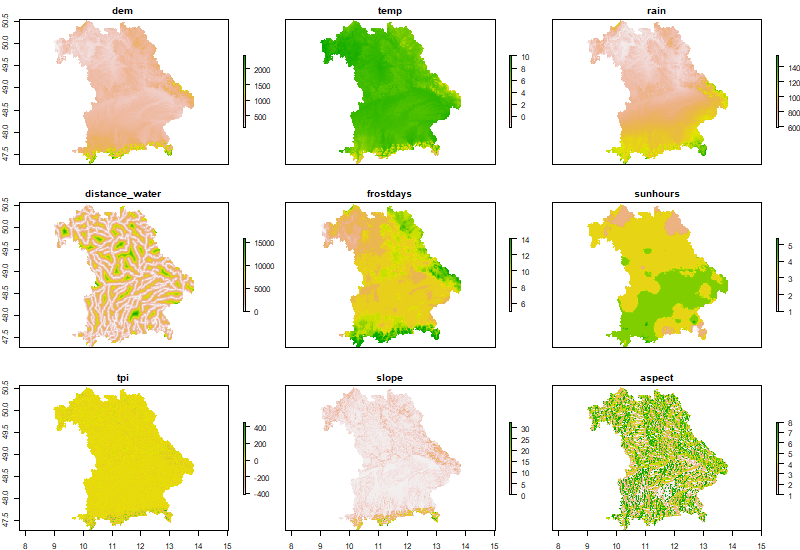
\includegraphics[width = 15cm, height = 12.5cm]{Figures/predictorstack.png}
    \caption{Plots der Variablen die für die Konstruktion des Datensatzes verwendet wurden. Zugang und Aufbereitung der Daten werden in Kapitel 2 behandelt.}
    \label{predictorstack}
\end{figure}
\newpage

\section{Daten: Zugang und Aufbereitung}
\label{section:Datenaufbereitung}
    Dieser Abschnitt behandelt Datenzugang und Aufbereitung. Es wird erläutert wie der zum Schätzen der Modelle gebrauchte Datensatz konstruiert wurde und woher die benutzten Prädiktorvarialben kommen. Auch werden Probleme beim beschriebenen Vorgehen angesprochen und mögliche Lösungsansätze vorgeschlagen.

\subsection{Bayern in der Vorgeschichte}
Datenbasis dieser Arbeit sind die Koordinaten archäologischer Fundstellen aus der Vorgeschichte. Peer Fender stellte diesen Datensatz 2016 im Rahmen einer GIS-gestützten Analyse der Siedlungslandschaft Bayerns mit dem Einsatz von Open Data für eine Dissertation zusammen. \cite{fender2017bayern} Dieser Datensatz ist nun für Studenten der LMU unter \cite{Datenbank} frei zugänglich und soll dazu dienen, die Studierenden in die Methoden der Analyse räumlicher Daten mit standard Geoinformationssystemen wie QGIS, SAGA oder GRASS-GIS einzuführen. Die Datenbank enthält über 27000 Einträge von Fundstellen innerhalb Bayerns aus der Bronze-, Eisen- und Späteisenzeit. Natürlich sind nicht nur die Orte an denen Funde gemacht wurden von Interesse, neben Koordinaten im World Geodetic System 1984 (WGS 84) sind Informationen zu Art der Fundstellen wie ``Siedlung'' oder ``Grab'', die Epoche in welche sich die jeweiligen Fundorte einordnen lassen, Höhe über dem Meeresspiegel und viele weitere Kovariablen enthalten. Die weitere Analyse beschränkte sich auf Fundstellen aus der Eisenzeit (Hallstatt- \& La Tènezeit; ca. 800 v. Chr. bis 50 n. Chr.), sowie die folgenden Variablen: 
\begin{itemize}
    \item Höhe über Normalnull
    \item Hangneigung, Hangausrichtung und Topographischer Position Index
    \item Wassernähe 
    \item Durchschnittliche Frosttage pro Jahr
    \item Durchschnittliche Jahrestemperatur
    \item Durchschnittliche Niederschlagsmenge
    \item Durchschnittliche Sonnenstunden pro Tag pro Jahr
\end{itemize}
Diese Variablen wurden ausgewählt, da sie naheliegend zur Modellierung der Habitateignung für eisenzeitliche Menschen erschienen. Klimaeinflüsse wie Temperatur und Niederschlag nehmen Einfluss auf potentielle Nahrungsquellen, Hangneigung und Hangausrichtung und elevationsbaiserte Maße sind von besonderem Interesse, da mit Beginn der Sesshaftigkeit in der Jungsteinzeit auch ein Überblick über ein Siedlungsumfeld relevant für die Wahl eines Niederlassungsortes wurde. \cite{sesshaft} Obwohl das Graben von Brunnen in der Eisenzeit weit verbreitet war, und damit die Nähe zu Gewässern unter Umständen keine Priorität mehr bei der Siedlungswahl darstellte, schien es durchaus sinnvoll zumindest die Distanz zu größeren Gewässern mit in die Analyse einzubeziehen. Siedlungen und Städte sind bis heute vom Trinkwasserzugang und den Transportmöglichkeiten von Gewässern abhängig; außerdem stellte das erzeugen eines Gewässerdistanz-Rasterlayers in R eine interessante Herausforderung dar. \\
Allerdings ergab sich für die weitere Analyse das Problem, dass für etablierte Klassifikationsverfahren wie ein logistisches Modell sowohl Präsenzdaten, also die Ausprägungen der Kovariablen an den Fundstellen, als auch Nonpräsenzdaten, also Werte der interessierenden Variablen an Orten die nicht im Datensatz von Fender enthalten sind, benötigt werden. Eine Möglichkeit dieses Problem zu lösen wäre es, die Daten für Bayern anhand der vorhandenen Messwerte zu interpolieren, und dann an den gewählten Nonpräsenzpunkten die Werte zu messen. Wie in Abbildung \ref{shinyfinal} erkennbar, sind die Sites (Blau) nicht homogen über das gesamte Untersuchungsgebiet verteilt. Dies macht deutlich, dass beispielsweise die Interpolation von Höhen- und Temperaturwerten in Gebirgsnähe nicht mehr trivial zu bewerkstelligen ist, weil sich diese Höhengebiete mit vergleichsweise geringen Temperaturen im Falle Bayerns größtenteils in Grenznähe befinden. Die Mehrheit der Fundstellen (``Sites'') liegt zentraler, im weiten Umfeld der Donau und ihrer Zuflüsse, was bewirkt das für Nonpräsenzpunkte (``Nonsites'') unter großer Ungenauigkeit extrapoliert werden müsste. Das genaue Vorgehen bei der Auswahl von Nonsites wird im Abschnitt zu Pseudo-Nonpresence-Sampling erklärt. \\
Eine bessere Möglichkeit zur Bewältigung des Nonsiteproblems bietet die manuelle Konstruktion eines ``vollständigen'' Datensatzes. Import und Manipulation georeferenzierter Vektor- und Rasterdaten lassen sich in R durch Pakete wie sf \cite{simplefeatures} und raster \cite{raster} mühelos durchführen, was es erlaubt, die Daten von Fender an den gewünschten Positionen zu vervollständigen bzw. einen ``kompletten'' Rasterdatensatz für ganz Bayern zu erstellen und aus diesem benötigte Werte an gewünschten Positionen zu extrahieren. Weil bis auf die minimale Wassernähe alle Variablen von Interesse frei und unkompliziert im Internet verfügbar sind, und weil es sich für spätere Resamplingverfahren und Visualisierungen besser eignet, wurde ein Rasterstack konstruiert aus dem benötigte Messwerte extrahiert wurden. 

\subsection{Rasterdaten}

Um zu gewährleisten, dass alle Rasterlayer die gleichen Ausmaße haben, wurden zunächst die bayrischen Ländergrenzen benötigt. GADM, \cite{GADM.org} eine globale Datenbank administrativer Ländergrenzen eignete sich für diesen Zweck. Die Funktion ``raster::getData'' erlaubt den direkten Import von Vektor- und Rasterdaten aus verschiedenen Datenbanken. In Kombination mit drei Zeichen ISO-Code und der administrativen Ebene (Staat, Bundesland, Landreis etc.) ließ sich so das gewünschte Areal zuschneiden. Eine genaue Erklärung zum Import und der Manipulation von Rasterdaten enthält Kapitel 2 von \cite{lovelace2019}. Im nächsten Schritt wurde ein mit zufälligen Werten vollgeschriebenes Raster erzeugt, welches zum ``masking'' der anderen Daten verwendet wurde. So lassen sich mit den Funktionen ``crop'' und ``mask'' aus dem Raster Paket geographische Daten auf das benötigte Maß zuschneiden. Allgemein wurde für die Konstruktion des Rasterstacks der für die Analyse verwendet wurde nach folgendem Schema verfahren: \\
\begin{enumerate}
    \item Suche nach frei zugänglichen Onlinedaten für gewünschte Variable
    \item Import der Daten in R
    \item Zuschneiden der Daten mit der vorab definierten Maske
    \item Plotten des Rasterlayers um zu prüfen ob Schritte 2 \& 3 erfolgreich waren
\end{enumerate}
Die Höhendaten, das sog. ``Digital Elevation Model'' (DEM) konnten auch via raster::getData importiert werden. Das DEM basiert auf Fernerkundungsdaten die im Jahre 2000 von der Shuttle Radar Topography Mission (SRTM) erhoben wurden. \cite{srtm} Die Auflösung von 90 Metern bildet einen sinnvollen Ansatz für den Rest der Analyse, da die von Fender gesammelten Daten zum größten Teil errechnete Mittelwerte aus einem Radius von 50m um die Fundstellen sind. Für das weitere Vorgehen wurde sich daher an einer Rasterauflösung von 90m pro ``Pixel'' orientiert. \\
Auch Temperatur- und Niederschlagsdaten konnten ähnlich importiert werden. WorldClim Version 2 enthält durchschnittliche monatliche Klimadaten für minimale, mittlere und maximale Temperatur sowie für Niederschlagsmengen der Jahre 1970-2000. \cite{Worldclim2} Aus dieser Datenbank konnten die Daten für Bayern auch via raster::getData importiert werden. \\
Hangneigung, Hangrotation und Topographic Position Index (TPI) mit der in ``raster'' enthaltenen Funktion ``terrain'' aus dem DEM errechnet. Für Neigung und Rotation folgt diese Prozedur dem in \cite{hillshading} beschriebenen Algorithmus basierend auf den Werten der 8 umgebenen Nachbarzellen der Rasterzelle deren Wert errechnet werden soll. TPI ist die Differenz zwischen dem Wert einer Zelle und dem Mittelwert ihrer 8 umgebenden Zellen. Diese Werte können auch, wie in der Dokumentation der Funktion ``terrain'' beschrieben, durch eine focal Operation auf den Rasterdaten errechnet werden. \cite{terraindoku} Sowohl Hangneigung als auch Rotation werden in Grad angegeben. Um die Werte für Hangrotation leichter interpretierbar zu machen wurden diese in einen Faktor mit 8 Ausprägungsstufen konvertiert. Eine Ausprägung von 1 entspricht einer Hangrotation Richtung Norden, eine Ausprägung von 2 Nordosten und so weiter. \\
Die durchschnittliche Anzahl von Frosttagen pro Jahr, sowie die durchschnittliche Anzahl Sonnenstunden pro Tag pro Jahr wurden vom Geoserver des deutschen Wetterdienstes in Form von TIFF Files heruntergeladen und mit der Funktion ``raster::raster'' in Rasterlayer umkonvertiert.\cite{frosttage} \cite{sonnenstunden} In Abbildung \ref{predictorstack} ist das Resultat des Datenimports zu erkennen. Auch in Abbildung \ref{predictorstack} zu sehen, ist der errechnete Rasterlayer, welcher die minimale Entfernung zum nächstgelegenen Gewässer eines jeden Pixels enthält. Wie dieser erzeugt wurde wird im nächsten Abschnitt erläutert. 

\subsection{Gewässer}

Ein sehr mächtiges Werkzeug für Rasterprocessing in R sind die Schnittstellen zu anderen Geoinformationssystemen. Auf Basis von Elevationsdaten lassen sich in GIS allerlei weitere Terraineigenschaften ableiten. So kann über die Schnittstelle zu GRASS GIS mit den Funktionen ``r.stream.extract'' und ``r.stream.distance'' aus einem DEM ein Abflussnetzwerk abgeleitet und im Anschluss daran die Entfernungen von jeder Rasterzelle zu diesem Netzwerk errechnet werden. Leider hatte das DEM aus dem Rasterstack eine zu geringe Auflösung um auf diesem Weg zu sinnvollen Ergebnissen zu kommen. So ließen sich nur die größten Donauzuflüsse und die Donau selbst auf diesem Weg aus dem Höhenmodell errechnen, was als unzureichend eingestuft wurde. \\
Als nächstes wurde versucht eine Funktion zu schreiben, welche für eine beliebige Liste vordefinierter Punkte die minimalen Distanzen zu den in einem Vektordatensatz enthaltenen Flüssen und Gewässern errechnet. Das verwendete Gewässernetz wurde einem online verfügbaren Shapefile entnommen. \cite{rivershapes} Grundidee war hier, die zentralen Koordinaten einer jeden Rasterzelle des Bayernrasters zu entnehmen, die minimalen Distanzen dieser zum Gewässershapefile mit ``geosphere::dist2line'' \cite{dist2line} zu ermitteln und im Anschluss einen Rasterlayer mit allen Distanzen zu rekonstruieren. \\ Obwohl die Ergebnisse vielversprechend aussahen, wurde sich gegen diese Methode entschieden. Grund dafür war unter anderem die hohe Rechenzeit. Selbst nach Parallelisieren dauerte das Errechnen der minimalen Gewässerdistanzen für einzelne Koordinatenpunkte auf der verfügbaren CPU ca. 1.2 Sekunden. Die Gesamtzeit für alle etwa 240000 Rasterzellen hätte also fast 80 Stunden betragen. Natürlich wäre an dieser Stelle ein Profiling der Funktion gekoppelt an das Umschreiben zeitaufwendiger Codeabschnitte in C++ möglich gewesen, dies hätte allerdings den Rahmen der Arbeit gesprengt, da hier in erster Linie Geoprocessing behandelt werden soll. \\
Glücklicherweise lässt sich das am Anfang von Abschnitt 2.2 beschriebene Masking nicht nur zum Zuschnitt von Rasterlayern benutzen. Die für den Brute-Force Ansatz importierten Gewässershapefiles können auch als Maske genutzt werden. Im Anschluss daran können mit der Funktion ``distance'' aus dem raster Paket die minimalen Distanzen zu den Masken für einen ganzen Rasterlayer auf einmal berechnet werden. Als letztes wurden beide so erzeugten Layer für die Entfernungen zum Flussnetzwerk und die Distanzen zu übrigen Gewässern mit der Funktion ``min'' vereint. Da vorimplementierte Rastermethoden deutlich effizienter sind als Werte für einzelne Zellen sequenziell zu bestimmen benötigte diese Vorgehensweise nur etwa 90 Minuten Rechenzeit. \\
Alle Rasterlayer wurden zu einem Rasterstack zusammengefügt. Die Ausprägungen der Variablen für Sites und Nonsites wurden dann mit ``raster::extract'' \cite{extract} aus dem Stack extrahiert. Damit fehlte nur noch ein geeignetes Samplingverfahren für das Ziehen von Nonsitepunkten aus Bayern. Der nächste Abschnitt geht auf diese Problematik ein. 

\subsection{Pseudo-Nonpresence-Sampling}

Das Anwenden von Klassifikationsalgorithmen setzt natürlich eine Einteilung in mindestens zwei verschiedene Klassen voraus. Da der Datensatz von Fender nur Orte enthält an denen Funde gemacht wurden, müssen Nicht-Fundorte also ergänzt werden. Ein in \cite{lovelace2019} beschriebenes Verfahren ist das Ziehen zufälliger Punkte aus dem Forschungsgebiet als ``Pseudo-Nonpräsenzdaten''. Üblicherweise zieht man diese unter der Nebenbedingung, dass sie nicht in eine vordefinierte Bufferzone um die Fundstellen fallen dürfen. Stellt man sich vor, dass Siedlungen im Allgemeinen nicht nur von einzelnen Individuen bewohnt werden und sich der Einflussbereich einer Siedlung nicht auf einen einzigen Punkt konzentriert, macht Bufferzone-Sampling intuitiv Sinn. Allerdings ist die optimale Wahl des Bufferradius nicht trivial. Wird der Radius zu klein gewählt, fallen also die Nonsites unter Umständen zu nah an Sites, so fallen die Ausprägungen beider Klassen aufgrund der räumlichen Korrelation in den Daten sehr ähnlich aus, was zur Folge hat, dass Klassifikationsverfahren überproportional hohe Fehlerraten produzieren. Wird der Radius dagegen zu groß gewählt, so fallen die Ausprägungen beider Klassen überproportional unähnlich aus, was unrealistisch niedrige Fehlerraten zur Folge hätte. Eine weitere Diskussion der Problematik räumlicher Korrelation findet sich in Abscnitt 3.4. Eine Visualisierung des Bufferradiusproblems ist in Abbildung \ref{shinyfinal} zu sehen. \\
Als sinnvoller Mittelweg bot sich ein Bufferradius von 1500 Metern um die Fundstellen an. Nicht nur erlaubt ein ähnlicher Radius moderate False-Positive- \& False-Negative-Rates beim Einschätzen der Modellperformance, auch geht man für die jüngere Eisenzeit in Nordfrankreich davon aus, dass etwa alle 3 km ein Gehöft (ein Einzelhof, einzelnes bebautes Grundstück) lag. \cite{nordfrankreich} Daher wurde davon ausgegangen, dass sich dieser ``Durchmesser'' des Einflussbereiches eisenzeitlicher Siedlungen auch auf andere fruchtbare Gebiete wie das Erdinger Land übertragen lässt. \\
Insgesamt waren nach der Einschränkung auf Fundstellen aus der Eisenzeit und dem Entfernen doppelter Einträge aus dem Datensatz noch 6174 relevante Sites übrig. Für das Schätzen der Modelle wurde die gleiche Menge Nonsites wie hier beschrieben aus Bayern gezogen, also basieren die Resultate auf einem Datensatz mit mehr als 12000 Einträgen. 

\subsection{Visualisierung mit Shiny}

Das Bufferradiusproblem kann innerhalb einer R-Shiny Applikation interaktiv untersucht werden. Zu sehen sind die mit dem Logit-Modell geschätzten predictive maps, die Sites (Blau) sowie die unter der Nebenbedingung des eingestellten Mindestabstandes gezogenen Nonsites in (Rot). Erkennbar wird, dass mit wachsendem Bufferradius die Nonsites in Richtung der Gebirge des Bayrischen Waldes und der Alpen abgedrängt werden. Dies hat zur Folge, dass sich der AUC Wert (Ein Maß für die predictive Performance eines Klassifikators) für wachsenden Bufferradius 1 annähert. Daraus folgt also, dass der gewählte Radius direkten Einfluss auf die Performance der Klassifikatoren nimmt. Auf AUC als Performancemaß für die prädiktive Güte wird in Abschnitt 3.4 näher eingegangen. 
\begin{figure}[H]
    \centering
    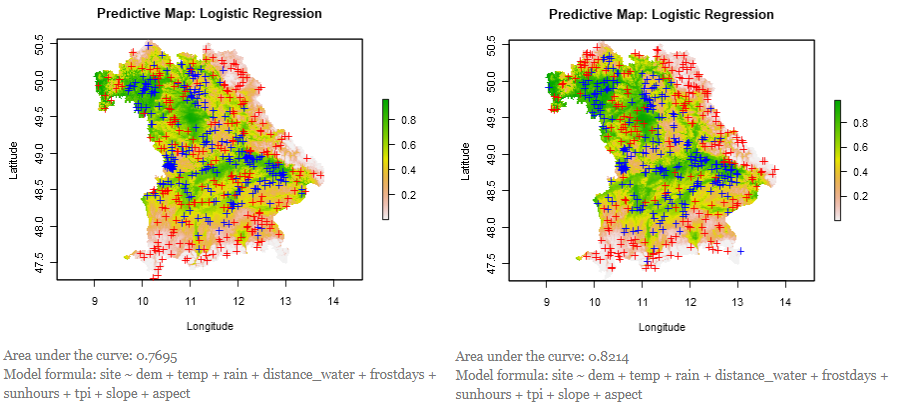
\includegraphics[width = 15cm, height = 7.5cm]{Figures/shinyfinal.png}
    \caption{Visualiserung der Lage von Sites und Nonsites. Links: Bufferradius 1500m. Rechts: Bufferradius 3000m.}
    \label{shinyfinal}
\end{figure}
\newpage

\section{Verwendete Klassifikatoren}
\label{section:Theorie}
Dieses Kapitel beschäftigt sich mit der Theorie aller verwendeten Klassifikatoren. Es wird aufgrund der Resultate des logistischen Modells argumentiert, dass die Datenauswahl weitgehend sinnvoll ist. Abschnitt 3.4 führt zudem die Ideen der verwendeten Cross Validation Strategien auf, mit denen die Performance der Modelle verglichen wurde. 

\subsection{Das logistische Modell}
Als Basismodell an dem die Performance der beiden anderen Classifier gemessen werden sollte, wurde ein logistisches Modell geschätzt. Das logistische Regressionsmodell entsteht aus dem Wunsch heraus, die Posteriorwahrscheinlichkeiten der K Klassen über lineare Funktionen im Predictorspace zu modellieren und gleichzeitig sicherzustellen, dass sie zu eins summieren und innerhalb des Intervalls [0,1] bleiben. \cite{logit}
Existieren nur zwei verschiedene Klassen in den Daten, zum Beispiel Sites und Nonsites, so lässt sich das logistische Modell mit nur einer linearen Funktion spezifizieren. Dem sog. linearen Prädiktor $\eta$. \\
\begin{equation}
    \eta = \beta_{\text{0}} + \beta_{\text{1}} \cdot {\text{Höhe}}  + \beta_{\text{2}} \cdot  {\text{Temp}}  + ... + \beta_{\text{p}} \cdot {\text{Hangausrichtung}} 
\label{eqlogit}
\end{equation}
Dabei gilt aus der Konstruktion von $\eta$ über die logarithmierten Chancen (log-odds):\\ 
\begin{equation}
\log \frac{\operatorname{Pr}(K=1 | X=x)}{\operatorname{Pr}(K=2 | X=x)}= \eta
\label{logodds}
\end{equation}
So müssen die aus dieser Konstruktion erhaltenen Koeffizienten anhand der log-odds, oder nach Exponentieren von $\eta$ anhand der Odds interpretiert werden. An dieser Stelle sollte angemerkt werden, dass es in dieser Arbeit nicht im Focus lag die Modelle optimal an die Daten anzupassen, um die zugrunde liegenden datengenerierenden Prozesse bestmöglich zu erklären. Daher wurden die Prädiktoren nur einzeln, als lineare Terme frei von Interaktionen in die Modelle aufgenommen. Die Resultate des logistischen Modells befinden sich in der folgenden Tabelle. 
\begin{table}[htb]
\centering
\begin{tabular}{llllll}
\hline
               & Estimate   & Sig. & Hangrotation & Estimate   & Sig.\\
Intercept      & -1.171e+01 & ***       & Nordost      & -1.591e-01 & *         \\
DEM            & -1.231e-03 & **        & Ost          & -3.988e-01 & ***       \\
Temperatur     & 1.421e+00  & ***       & Südost       & -1.568e-01 & *         \\
Niederschlag   & -4.150e-03 & ***       & Süd          & -2.733e-01 & ***       \\
Gewässer Dist. & -3.102e-05 & ***       & Südwest      & -3.438e-01 & ***       \\
Frosttage      & 2.612e-01  & ***       & West         & -1.876e-01 & *         \\
Sonnenstunden  & 6.659e-01  & ***       & Nordwest     & -8.278e-02 &           \\
TPI            & 1.787e-03  &           &              &            &           \\
Hangneigung    & -1.378e-01 & ***       &              &            &           \\
\hline
\end{tabular}
\caption{Geschätzte Koeffizienten des Logit-Modells. Nonsites und Sites sind als 0/1-kodierte Variable in das Modell eingeflossen. Sig. Codes: 0 ‘***’ 0.001 ‘**’ 0.01 ‘*’ 0.05 }
\label{tab:basefitcoeffs}
\end{table} \\
Im Allgemeinen lassen sich die geschätzten Koeffizienten am schnellsten über ihre Vorzeichen interpretieren. Ein negatives Vorzeichen bedeutet, dass, ceteris paribus, ein Steigen der entsprechenden Kovariable eine Senkung der log-odds für Klasse 1 (hier Sites) zur Folge hätte. Dies ist hier für die Variablen Hangneigung, Gewässerdistanz, Niederschlag, DEM (Höhe über N.N.) der Fall und erscheint bei einem Blick auf die Prediktorkarten in Abbildung \ref{predictorstack} und die geographischen Häufungen der Sites durchaus sinnvoll. So würde man erwarten, dass bei Annäherung an die Alpen -- also Steigern der Höhe, die Chancen bei einer Ausgrabung fündig zu werden sinken. Ein positives Vorzeichen bedeutet hingegen, dass eine Steigerung der entsprechenden Kovariable eine Steigung der log-odds für Klasse 1 (Sites), unter Konstanthalten der anderen Variablen, zur Folge hätte. Dies ist hier sowohl für die Anzahl durchschnittlicher Sonnenstunden pro Tag pro Jahr, als auch für die durchschnittliche Anzahl Frosttage pro Jahr der Fall. (TPI hat mit einem p-Wert von weit über 5\% keinen signifikant von 0 verschiedenen Einfluss auf die log-odds.) Interessant ist auch, dass alle Hangrotationskoeffizienten ein negatives Vorzeichen besitzen. Dies könnte unter Umständen aus dem Zusammenhang von Hangrotation, Hangneigung und Höhenmodell erklärt werden. So können nur an Stellen an denen das Höhenmodell Hänge besitzt Werte für die Hangrotation ermittelt werden. Um diesen Zusammenhang zu klären, sollten noch weitere Untersuchungen durchgeführt werden. \\
Insgesamt scheint die Variablenauswahl sinnvoll, nur der TPI ist trotz der Stichprobengröße von mehr als 12000 Sites und Nonsites nicht signifikant. 
Anmerkung: Während die logit-Transformation des linearen Prädiktors häufig mit der sigmoiden Form der logistischen Funktion in Verbindung gebracht wird, sollte nicht unerwähnt bleiben, dass die logistische Regression zur Klassifikation den Prädiktorraum je nach festgelegter Entscheidungsgrenze mit einer Hyperebene in (in diesem Fall) zwei Klassengebiete unterteilt. \cite{trenngerade} Dies soll mit Abbildung \ref{trenngerade} veranschaulicht werden. 

\begin{figure}[H]
    \centering
    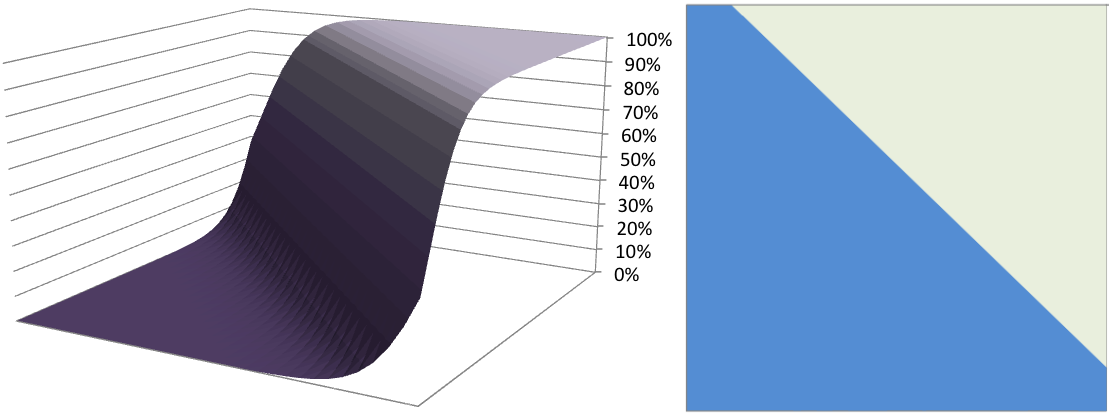
\includegraphics[width = 13cm, height = 7cm]{Figures/trenngerade.png}
    \caption{Logistische Regression mit zwei Kovariablen. Links: Sigmoide Form der auf zwei Variablen angepassten logistischen Funktion. Rechts: Lineare Trenngerade bei einer Entscheidungsgrenze von 50\%. \cite{trenngerade}}
    \label{trenngerade}
\end{figure}

Dieser bemerkenswerte Zusammenhang wirft die Frage auf, ob sich, unabhängig von der Definition über log-odds, lineare Trennebenen im vieldimensionalen Prädiktorraum finden lassen. Der nächste Abschnitt beantwortet diese Frage und führt sog. Kernel-Methoden ein um diese Methoden auf den nicht linear trennbaren Fall auszuweiten.

\subsection{Support Vector Machines}
\subsubsection{Linear separierende Hyperebenen}
Es ergibt sich, dass via logistischer Regression eine lineare Trennebene zur Klassifikation ermittelt werden kann. Dieser Abschnitt befasst sich mit der Konstruktion von linearen Hyperebenen zur Klassentrennung. Dieses Verfahren versucht die Daten so optimal wie möglich in verschiedene Klassen zu zerlegen. Es bildet die Grundlage für Support Vector Classifier. \cite{hyperplanes}\\
Sei L eine Hyperebene definiert durch die Gleichung
\begin{equation}
    f(x)=\beta_{0}+\beta^{T} x=0
\label{eqhyperplane}
\end{equation}
Im zweidimensionalen Fall ergibt sich eine Trenngerade. Es lässt sich zeigen:
\begin{enumerate}
    \item Für beliebige Punkte $x_{1}$ und $x_{2}$ in L gilt: $\beta^{T}\left(x_{1}-x_{2}\right)=0$ und daher ist der Normalenvektor von L gegeben durch: $\beta^{*}=\beta /\|\beta\|$
    \item Für jeden Punkt $x_{0}$ in L gilt: $\beta^{T} x_{0}=-\beta_{0}$
    \item Der Abstand eines punktes $x$ zu L ist gegeben durch: \\
    $\beta^{* T}\left(x-x_{0}\right)=\frac{1}{\|\beta\|}\left(\beta^{T} x+\beta_{0}\right)=\frac{1}{\left\|f^{\prime}(x)\right\|} f(x)$
\end{enumerate}
Daher ist $f(x)$ proportional zum Abstand von $x$ zur Hyperebene definiert durch $f(x)=0$. \cite{hyperplanes}\\
Grundsätzlich versuchen auf Trennebenen basierte Lernalgorithmen die Abstände der fehlklassifizierten Punkte zur Trenngerade zu minimieren. Um diese Abstände optimieren zu können muss allerdings zunächst eine Startebene festgelegt werden. Dies bring jedoch mit sich, dass im linear trennbaren Fall (keine Fehler bei der Klassifikation) mehrere optimale Trennebenen existieren können. Welche gefunden wird hängt von der Startposition ab. Auch würden Algorithmen wie \textit{stochastic gradient descent} im nicht linear trennbaren Fall nicht konvergieren. \cite{hyperplanes} Im Falle von nicht linear separablen Daten lassen sich trotzdem lineare Trennebenen durch Basistransformation der originalen Daten in einen höherdimensionalen Raum konstruieren. Eine einzigartige Lösung lässt sich beispielsweise durch Maximieren der ``Marginbreite'' also des Bereiches um die Trennebene in dem keine Punkte liegen kalkulieren. Dieser Bereich wird vollständig durch die Punkte definiert, welche sich am nächsten an der Ebene befinden. Nach \cite{hastie01statisticallearning} ergibt sich, dass der Lösungsvektor der Ebene als Linearkombination dieser ``Support Points'' definiert werden kann. Dies bildet die Grundlage für die im nächsten Abschnitt diskutierten Support Vector Classifier. 

\subsubsection{Support Vector Classifier}

\begin{figure}[H]
    \centering
    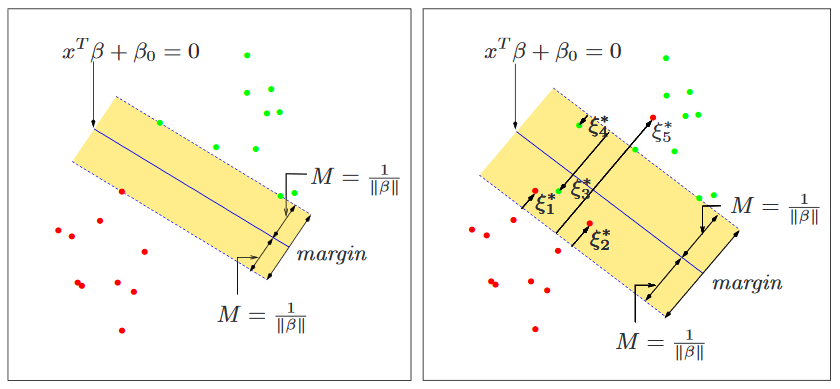
\includegraphics[width = 13cm, height = 7cm]{Figures/svmargin.PNG}
    \caption{Support Vector Classifier. Links: Der im Featurespace linear trennbare Fall. Die Trennebene ist die durchgezogene Linie, während gestrichelte Linien die maximale Margin der Breite $2M=2/\|\beta\|‖$ eingrenzen. Rechts: Der nicht linear trennbare Fall. Die mit $\xi_{j}^{*}$ bezeichneten Punkte befinden sich um einen Betrag $\xi_{j}^{*}= M \xi_{j}$ auf der falschen Seite ihrer Margin. Für Punkte auf der richtigen Seite ist $\xi_{j}^{*}=0$. Die Breite der Margin wird unter der Nebenbedingung $\sum \xi_{i} \leq \text {constant}$ maximiert. $\sum \xi_{j}^{*}$ ist die Gesamtdistanz der Punkte auf der falschen Seite der Trennebene.\cite{svclassifier}}
    \label{svclassif}
\end{figure}

Überlappen sich die Punkte im Featurespace gibt es zwei intuitive Möglichkeiten die Nebenbedingung in \ref{svclassif} zu formulieren. Als erstes könnte die Summe der absoluten Gesamtdistanzen konstant gehalten werden, dies ist aber im Allgemeinen kein konvexes Optimierungsproblem. Daher wird der ``standard'' Support Vector Classifier unter der Randbedingung die proportionalen Anteile der falschen Klassenzuweisungen unter einem Maximum zu halten formuliert. 
\begin{equation}
    \label{eqsvmoptim}
    y_{i}\left(x_{i}^{T} \beta+\beta_{0}\right) \geq M\left(1-\xi_{i}\right)
\end{equation}
Der Wert $\xi_{i}$ in der Nebenbedingung $y_{i}\left(x_{i}^{T} \beta+\beta_{0}\right) \geq M\left(1-\xi_{i}\right)$ entspricht dem relativen Anteil mit dem die vorhergesagte Klasse $f\left(x_{i}\right)=x_{i}^{T} \beta+\beta_{0}$ des Punktes $x_{i}$ von der durch die Entscheidungsgerade geschätzten Klasse abweicht. Daher wird durch Einschränken von $\sum \xi_{i}$ der gesamte relative Betrag, um den Prognosen auf der falschen Seite ihrer Marge fallen, eingeschränkt. Falsche Klassifizierungen treten auf wenn $\xi_{i}>1$ also wird durch Begrenzen der Summe  $\sum \xi_{i}$ die maximale Anzahl von Trainingsfehlern auf den gleichen Wert begrenzt. \cite{svclassifier}

Die optimale Breite der Margin eines Support Vector Classifiers muss unter weiteren Nebenbedingungen wie beispielsweise bestmöglicher Prognoseperformance für unbekannte Daten oder vergleichbaren Kriterien bestimmt werden. Dieser Kostenparameter $C$ ist also verantwortlich dafür, wie stark der Einfluss von weit von der Trennebene entfernten Punkten auf die Lage dieser ist. Große Werte für $C$ optimieren die Trennebene eher für korrekt klassifizierte Punkte nahe der Ebene. Kleinere Werte verstärken eher den Einfluss von Punkten die weiter von der Trennebene entfernt liegen. \cite{svclassifier} \\
Mit welcher Strategie Hyperparameter wie $C$ vor dem Fitten des Modells bestimmt werden, wird in Abschnitt 3.4 erklärt.  

\subsubsection{Kernel-Methoden und Support Vector Machines}

Die bisher beschriebene Support Vector Methodik beschränkt sich auf das Finden linearer Trennebenen im originalen Predictorspace. Werden durch das Berücksichtigen von Punkten innerhalb einer vordefinierten Grenzregion um die Entscheidungsebene auch nicht komplett linear trennbare Fälle schätzbar, so existieren weiterhin eine Vielzahl von möglichen Datensituationen in denen ein einfacher SV-Classifier an seine Grenzen stößt. \\
Wie mit anderen linearen Modellen lässt sich die Methodik des SV-Classifiers durch Basistransformationen des Predictorspace erweitern. Diese Idee wird in Abbildung \ref{kerneltrick} visualisiert. 

\begin{figure}[H]
    \centering
    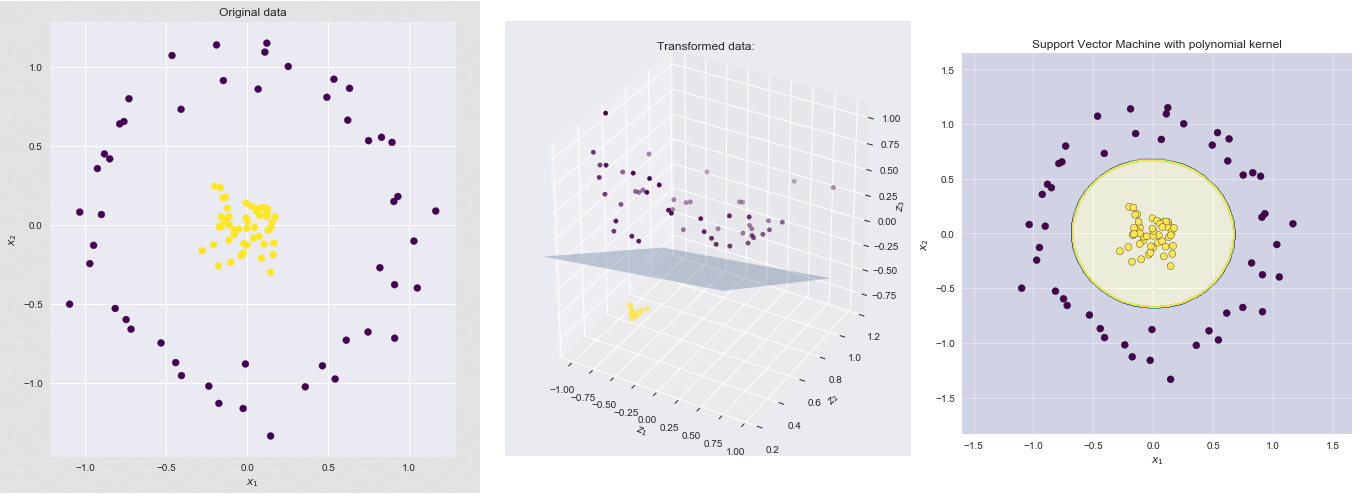
\includegraphics[width = 15cm, height = 6.5cm]{Figures/kerneltrick.png}
    \caption{Nichtlineares Klassifikationsproblem. Die im linken Panel abgebildete Datensituation lässt sich im originalen Predictorspace nicht linear trennen. Die in der Mitte abgebildete Transformation erlaubt die konstruktion eines linearen SV-Classifiers im neuen Prädiktorraum. Rechts ist die Trennlinie zu sehen welche sich durch Retransformieren der linearen Entscheidungsgrenze des 3D Raumes auf den ursprünglichen Prädiktorraum ergibt. \cite{kernelintuition} }
    \label{kerneltrick}
\end{figure}
Um komplexere, nicht-lineare Entscheidungsgrenzen zu erhalten, wird der ``Support Vector Machine'' Algorithmus angewendet. Dieser erlaubt es vieldimensionale Transformationen des Prädiktorraums zu betrachten. (In einigen Fällen kann die Dimension des Predictorspace bis ins Unendliche wachsen.) Dazu ersetzen wir $x$ überall in den bisherigen Formeln durch $\phi(x)$ und wiederholen den Optimierungsprozess. \cite{kernelintuition} Generell wird durch die Transformation der Daten in einen höherdimensionalen Raum die Berechnung von Abständen deutlich aufwendiger als beispielsweise im zweidimensionalen Fall. Um dieses und weitere Probleme zu umgehen, verwendet man für die Transformationen sog. ``Kernel'' oder ``Kern'' Funktionen. Eine intuitive Betrachtungsweise von Kernelfunktionen wäre, dass diese Funktionen entsprechen, welche messen, wie eng die Inputvektoren $x$ und $z$ miteinander verwandt sind. Wenn $x$ und $z$ ähnlich zueinander sind, gibt der Kernel also einen großen Wert aus, und wenn sie ungleich sind, liefert der Kernel kleinere Werte. Dies rechtfertigt die Verwendung eines Gaußkerns für die weitere Analyse. \\
\begin{equation}
    \label{gausskern}
    K(x, z)=\exp \left(-\frac{\|x-z\|^{2}}{2 \sigma^{2}}\right)
\end{equation}
Sind $x$ und $z$ gleich so nimmt der Gausskern den Wert 1 an. Je größer die Differenz von $x$ und $z$, desto mehr nähert sich der Wert des Gausskerns 0 an. \\ Für die Analyse der Eisenzeitfundstellen wurde ein Gausskern verwendet. Die optimale Bandbreite des Kerns ist ein weiterer Hyperparameter, der vor Schätzen des Modells angepasst werden muss. Dieser Parameter $\sigma$ bestimmt die Breite des Kerns, was sich direkt auf die Form der Entscheidungsgrenze auswirkt. Große Werte für $\sigma$ tragen dazu bei, dass die Grenze flexibel ist, was für Prognosemodelle eher ungünstig sein kann, da in solchen Fällen ``overfitting'' vermieden werden sollte.

\subsection{Regression Trees \& Random Forests}

Eine weitere Möglichkeit zur Klassifikation sind Decision Trees. Dieser Abschnitt führt die Theorie von binären Partitionierungen zum Aufbau von Regressions- und Klassifikationsbäumen an und beschäftigt sich mit der Generalisierung dieser Methodik, um robustere Prognoseergebnisse aus den Vorhersagen von Decision Trees zu erzeugen. 

\subsubsection{Regression Trees}

\begin{figure}[H]
    \centering
    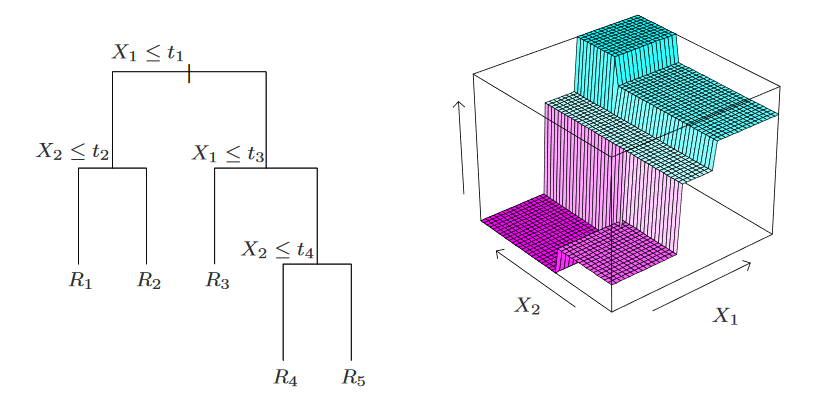
\includegraphics[width = 15cm, height = 6.5cm]{Figures/treesplit.PNG}
    \caption{Regressionsbaum. Links: Ein Beispiel für einen durch rekursive binäre Partitionierung eines zweidimensionalen Prädiktorraums erhaltenen Regression Trees. Rechts: Ein Diagramm der durch diese Einteilung erhaltenen Prognosefläche im Prädiktorraum. \cite{treesplit} }
    \label{treesplit}
\end{figure}

Allgemein lässt sich eine Outcomevariable $Y$ durch Unterteilen des Prädiktorraums in verschiedene Regionen und Zuweisen eines konstanten Wertes $Y^{*}$ zu jeder dieser Regionen modellieren. Da bestmögliche Teilregionen beliebig komplex, und daher schwierig zu charakterisieren, werden können beschränkt sich dieser Ansatz auf rekursive binäre Partitionen, was bedeutet, dass der Prädiktorraum zunächst in zwei Regionen aufgeteilt wird und der Outcome $Y$ mit dem Mittelwert von $Y$ jeder Teilregion modelliert wird. Die Variable nach der aufgeteilt wird, wird einem bestmöglichen Split entsprechend ausgewählt. Dann werden eine oder beide dieser Regionen in je zwei weitere Regionen aufgeteilt, und dieser Prozess wird fortgesetzt, bis eine vordefinierte Regel zum Anhalten in Kraft tritt. \cite{treesplit} Aus diesem Prozess ergibt sich die Baumstruktur im linken Panel von Abbildung \ref{treesplit}. Trotz der Restriktion auf binäre Splits lässt dieses Verfahren, in Abhängigkeit der gewählten Anhalteregel, beliebig viele Aufteilungen des Variablenraumes zu. Der größte Vorteil von Entscheidungsbäumen ist ihre simple Interpretierbarkeit. Das gesamte Modell ist in einem binären Baum enthalten, die einzige Schwierigkeit bildet die Interpretation der Baumstruktur bei vielen Splits und/oder vielen Kovariablen. \\
Für die Klassifikation der Eisenzeitsiedlung stellt sich also die Frage, wie genau der Entscheidungsbaum wachsen sollte um optimale Prognosen zu treffen. Der Datensatz besteht aus einem 2-Klassen Outcome (Sites vs. Nonsites) und 9 Einflussgrößen mit insgesamt über 12000 einzelnen Beobachtungen. Es muss also entschieden werden welche Variablen an welchen Stellen aufgeteilt werden und welche finale Struktur der Baum haben sollte. Angenommen der Prädiktorspace soll in $M$ Regionen $R_{1}, R_{2}, \ldots, R_{M}$ unterteilt werden und der Outcome des Modells wird als Konstante $ c_{m}$ in jeder Region modelliert. 
\begin{equation}
    \label{treemodel}
    f(x)=\sum_{m=1}^{M} c_{m} I\left(x \in R_{m}\right)
\end{equation}
So ergibt sich, ähnlich einem Mittelwertsmodell, der optimale Fit für die Klassifikation als Durchschnitt der Response in jeder der Teilregionen. 
\begin{equation}
    \label{leastsquarestree}
    \hat{c}_{m}=\operatorname{ave}\left(y_{i} | x_{i} \in R_{m}\right)
\end{equation}

Durch Minimieren der quadrierten Abstände der Punkte der Teilregionen zu den Mittelwerten der vorgeschlagenen Klassen lässt sich also für jeden binären Split ein optimaler Wert finden an dem die Aufteilung durchgeführt werden sollte. 
Dieser Prozess wird so lange wiederholt bis die gewünschte Größe bzw. Tiefe des Regressionsbaumes erreicht ist. Wie lange also das Splitting wiederholt werden sollte ist ein Hyperparameter der nicht ohne ein notwendiges Kriterium bestimmt werden kann. Bäume die den Prädiktorraum in zu viele kleine Partitionen unterteilen tendieren dazu, übermäßig viele Informationen aus dem ``Trainingsdatensatz'' zu lernen. Dieses Overfitting führt im Normalfall zu schlechteren Prognoseergebnissen auf ``Testdaten''. Für predictive maps die angeben an welchen Stellen die bayrische Landschaft als Habitat für Menschan aus der Eisenzeit geeignet ist, sind zu tiefe Bäume also eher nicht erstrebenswert. Wie oben erwähnt, besteht der verwendete Datensatz aus etwa 12000 Einträgen, die Prognosekarten werden also auf Basis von über 200000, dem Modell unbekannten, Rasterzellen generiert.\\ Die beste Strategie um einzelne Bäume zu optimieren ist ``cost-complexity pruning'' ein Verfahren, dass zunächst einen ``vollständigen'' Baum $T_{0}$ erzeugt um dann nach einem Teilbaum $T \subset T_{0}$ sucht, der das in \ref{costcomplexity} definierte cost-complexity Kriterium minimiert, also den Tradeoff zwischen Modellfit und Komplexität des Baumes zu optimieren versucht. \\
Sei $m$ die Anzahl an Endpunkten des Baumes $T_{0}$, also die Anzahl der Partitionen $R_{m}$ in die der Baum den Prädiktorraum einteilt. Sei außerdem $N_{m}$ die Anzahl der Beobachtungen $x_{i}$ im Endpunkt $R_{m}$ und $|T|$ die Anzahl der Endpunkte des Teilbaumes  $T \subset T_{0}$.
Mit \\
\begin{equation}
    \label{treecost1}
    \hat{c}_{m}=\frac{1}{N_{m}} \sum_{x_{i} \in R_{m}} y_{i}
\end{equation}
\begin{equation}
    \label{treecost2}
    Q_{m}(T)=\frac{1}{N_{m}} \sum_{x_{i} \in R_{m}}\left(y_{i}-\hat{c}_{m}\right)^{2}
\end{equation}
lässt sich das cost-complexity Kriterium definieren: 
\begin{equation}
    \label{costcomplexity}
    C_{\alpha}(T)=\sum_{m=1}^{|T|} N_{m} Q_{m}(T)+\alpha|T|
\end{equation}

Ziel ist es also, den Baum $T_{\alpha} \subset T_{0}$ zu finden welcher das CC-Kriterium $ C_{\alpha}(T)$ minimiert. Dies wird üblicherweise mit einer Mischung aus ``weakest link pruning'' und Cross Validation bewerkstelligt. \cite{treesplit} für eine detailliertere Erklärung dieser Methoden bzw. 3.4 Für eine Diskussion der verwendeten Verfahren zur Cross Validation. \\
Anmerkung: Das hier beschriebene Vorgehen mit Minimieren der quadratischen Abstände ist nur für Regression Trees geeignet. Für die Klassifikation wird im Normalfall eine Missklassifikationsmaß wie der Missclassification Error oder der Gini-Index minimiert. Der Vollständigkeit halber wurde hier die Konstruktion von Regressionsbäumen beschrieben, allerdings ist das Vorgehen für Klassifikationsbäume, abgesehen von der gewählten ``cost function'' identisch. 

\subsubsection{Random Forest Classifier}

Ein Nachteil einzelner Regressions- bzw. Klassifikationsbäume ist die hohe Variabilität der aus ihnen resultierenden Schätzungen. So kann eine minimale Veränderung im Datensatz eine drastische Veränderung der Baumstruktur zu Folge haben was also einen spürbaren Effekt auf die Prognosen von Trees haben kann. Die am weitesten verbreitete Methode zur Reduktion der Vorhersagevarianz ist ``bootstrapped aggregation'' also das Schätzen und Aggregieren vieler einzelner Entscheidungen auf Bootstrapstichproben. \\
Random forests sind eine Kombination einzelner Baumprädiktoren, so dass jeder Baum von unabhängig und identisch gezogenen Werten eines Zufallsvektors der Daten abhängt. Die durch Generalisieren des Random Forest auf Testdaten erhaltene Fehlerrate konvergiert mit wachsender Stückzahl der Trees im Random Forest fast sicher gegen einen Grenzwert. Dieser Generalisierungsfehler hängt von der Prognosestärke der individuellen Bäume und der Korrelation der Bäume untereinander ab. \cite{randomforest}\\
Grundsätzlich geht man zur Bildung eines Random Forest Classifiers nach dem folgenden Schema vor:
\begin{enumerate}
    \item Ziehe eine Bootstrap Stichprobe der Größe $N$ aus den Daten.
    \item Erzeuge einen Regressions- oder Klassifikationsbaum entsprechend des jeweils benötigten Kriteriums. (Cost Funktion)
    \item Wiederhole Schritte 1 und 2 so lange bis die gewünschte Zahl Bäume erreicht wurde. 
    \item Treffe Prognoseentscheidung für Regression anhand des Durchschnitts der Vorhersagen aller Bäume bzw. anhand der ``Mehrheit der Stimmen'' des Baumensembles für Klassifikation. 
\end{enumerate}
Anmerkung: Eine Prognosekarte die nur die erwarteten Klassen für jede Rasterzelle abbildet wäre im Zweiklassenfall nicht sonderlich hilfreich. Die Softwarepakete ``ranger'' \cite{ranger} und ``randomForest'' \cite{forestpackage} erlauben es allerdings auch die geschätzten Klassenzugehörigkeiten als Wahrscheinlichkeiten auszugeben. So sind auch die zugehörigen Prognosekarten zu Logit-Modell und SVM-Classifier zu interpretieren, wodurch die Karten alle direkt miteinander vergleichbar sind. Weitere Details zu Random Forest Klassifikatoren und Beweise dazu, dass dekorrelierte Baumensembles reduzierte Varianzen besitzen finden sich in \cite{randomforest}. 

\subsection{Hyperparameter Tuning \& Modellperformance}

Um die Klassifikatoren nicht nur visuell oder anhand geschätzter Zelldifferenzen miteinander vergleichen zu können und die Hyperparameter der SVM- und Random Forest Classifier zu bestimmen (tunen) wird üblicherweise 5- oder 10-fold Crossvalidation durchgeführt. Dabei wird der Classifier nur auf einem Teil des Gesamtdatensatzes trainiert und im Anschluss anhand der übrigen Testdaten und einem passenden Performancemaß getestet. Diese Schritte werden beliebig oft unter Variation der Hyperparameter wiederholt um den vordefinierten Parameterraum nach den optimalen Modellparametern zu durchsuchen. Als Maß für die Prognosegüte wurde hier die Fläche unter der ``receiver operating characteristic'' Kurve herangezogen. Diese ermittelt für jede Entscheidungs-Threshold vgl. \ref{trenngerade} im Intervall $[0,1]$ die False-Positive und False-Negative Raten. Die Fläche unter der Kurve kann also als Schätzer für die Gesamtprognosegüte verwendet werden. \\
Herkömmliche CV unterteilt den Datensatz zufällig in Trainings- und Testdaten. Punkte die auf der Erdoberfläche nahe beieinander liegen haben durch die stetige Natur geographischer Einflussgrößen sehr häufig ähnliche Variablenausprägungen. (Orte die nur einige hundert Meter voneinander entfernt sind ähneln sich im Allgemeinen in der Niederschlagsmenge und Durchschnittstemperatur) Dies hat zur Folge, dass bei Crossvalidation der Trainingsdatensatz Informationen über die Testdaten enthält wenn viele Punkte die ursprünglich nahe beieinander lagen in unterschiedliche Sets aufgeteilt werden. Daher wurde für die Modellperformance herkömmliche CV mit ``Spatial'' Cross Validation verglichen. Bei Spatial CV werden die Daten in räumlich zusammenhängende Stücke geteilt welche dann als Test- und Trainingssets verwendet werden. Abbildung \ref{resamplingviz} illustriert die Differenzen beider Methoden. 
\begin{figure}[H]
    \centering
    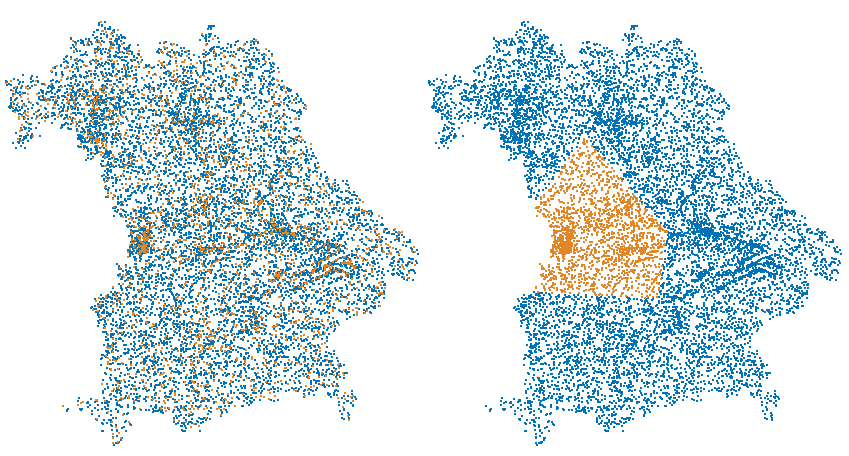
\includegraphics[width = 15cm, height = 6.5cm]{Figures/resampling.png}
    \caption{Resamplingverfahren. Links: Klassische Kreuzvalidierung -- Die Daten werden zufällig in Trainings- (Orange) und Testdaten (Blau) eingeteilt. Rechts: Spatial Cross Validation -- Die Daten werden auch in zwei Sets aufgeteilt, allerdings hängen diese Sets jeweils räumlich zusammen.}
    \label{resamplingviz}
\end{figure}
Eine räumlich zusammenhängende Aufteilung hat zur Folge, dass die Information über das Testset, welche im Trainingsset enthalten ist verringert wird. Also sollte erwartet werden, dass die mittleren Performanceergebnisse mit Spatial CV ein wenig nach unten korrigiert sind. Der Ergebnisvergleich der beiden Verfahren befindet sich in Kapitel 4. \\
Anmerkung: Die Verwendung derselben Daten für die Performanceschätzung und das Hyperparametertuning würde zu überoptimistischen Ergebnissen führen \cite{nestedresmpling2}. Dies kann durch nested Spatial CV vermieden werden. Folgende Grafik verdeutlicht das Vorgehen dabei: 
\begin{figure}[H]
    \centering
    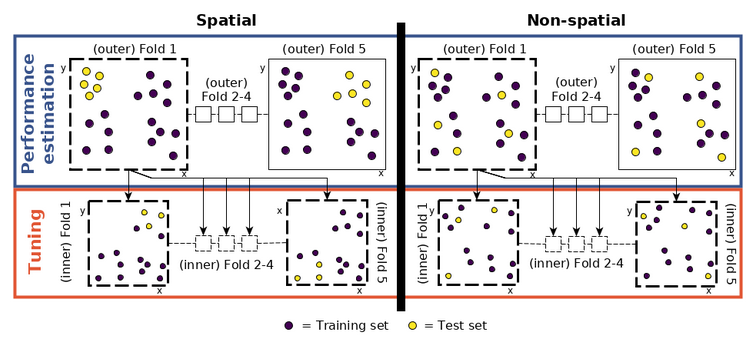
\includegraphics[width = 15cm, height = 6.5cm]{Figures/nestedresampling.PNG}
    \caption{Nested Resampling. Links: Die Unterteilung in räumlich zusammenhängende Stücke der spatial CV. Performance estimation wird auf äußeren Folds durchgeführt, optimale Hyperparameter werden durch erneute Unterteilung der äußeren Folds in Trainings- und Testdaten ermittelt. Rechts: Das gleiche Schema für herkömmliche CV. \cite{nestedresmpling2}}
    \label{nestedresamplingviz}
\end{figure}

\newpage

\section{Ergebnisse}

\label{section:Ergebnisse}
\subsection{Prognosekarten \& Cell Difference Maps}
\begin{figure}[H]
    \centering
    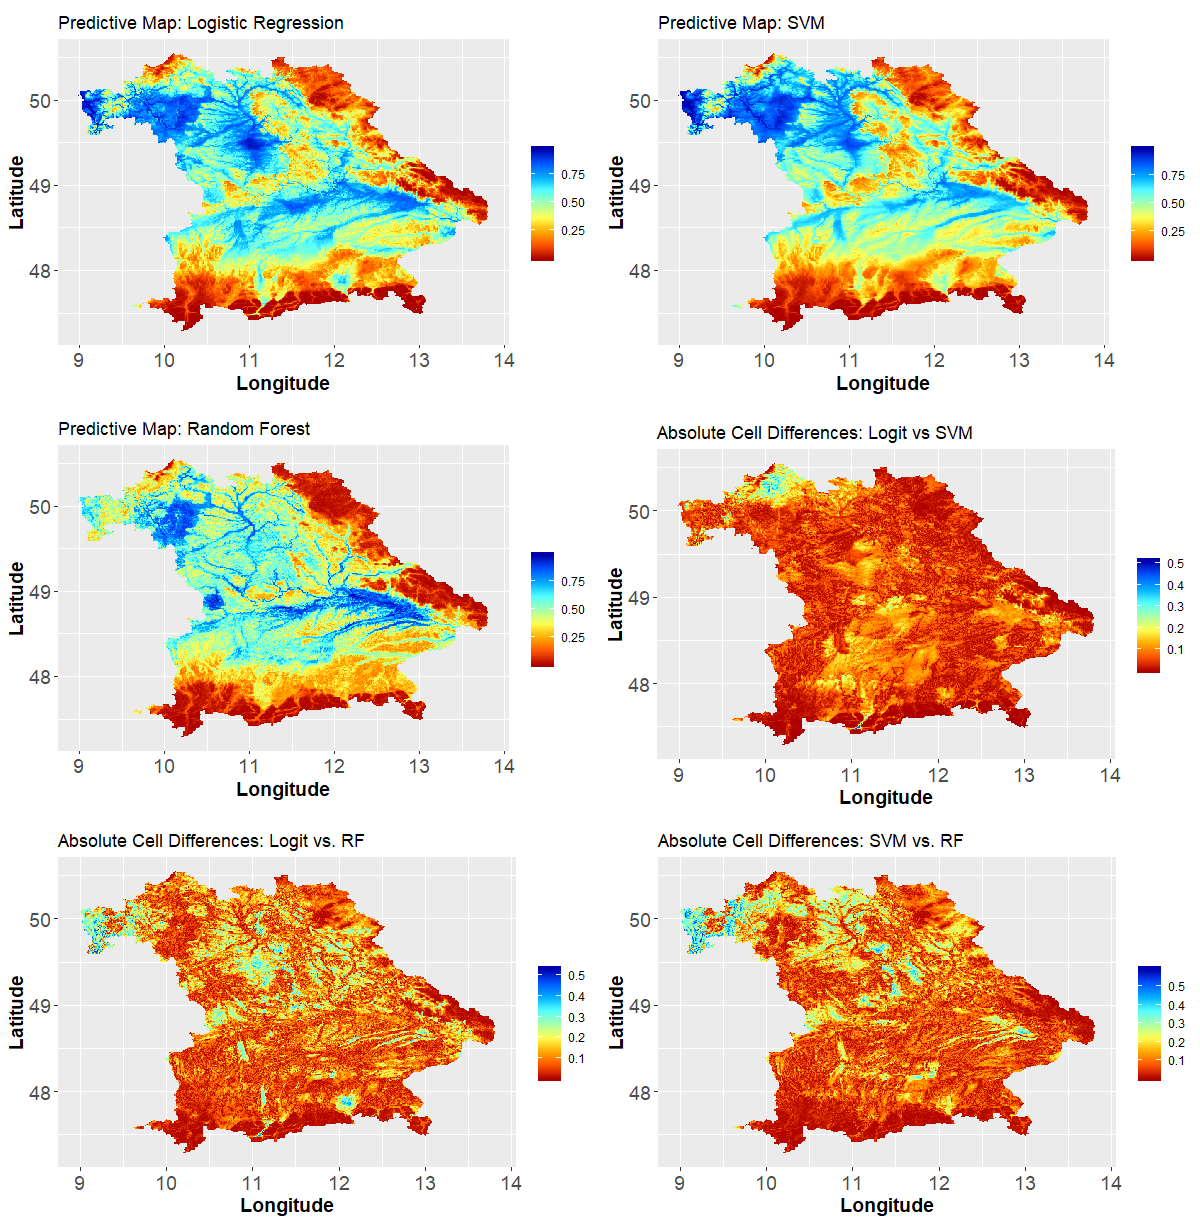
\includegraphics[width = 15cm, height = 19cm]{Figures/pmapsfinal.png}
    \caption{Die Prognosen der Modelle für den gesamten Rasterdatensatz. In den Karten oben links sind die geschätzten Wahrscheinlichkeiten für die Zugehörigkeiten der Rasterzellen zur Klasse ``Sites''. Die drei Karten in der unteren rechten Ecke visualisieren die absoluten Differenzen der Schätzergebnisse von Modell zu Modell.}
    \label{pmapsfinal}
\end{figure}
Eine praktische Eigenschaft von Rasterdaten ist die ``Vollständigkeit'' für das interessierende Areal. Im Normalfall müsste interpoliert werden um lückenlose Prognosen aufstellen zu können, da der Datensatz komplett aus Rasterlayern konstruiert wurde konnten so Vorhersagekarten für ganz Bayern generiert werden. Die Farbe der Karten kodiert die Wahrscheinlichkeit der Zugehörigkeit der einzelnen Pixel zur Klasse ``Site''. Rot lässt geschätzte Wahrscheinlichkeiten nahe 0 vermuten, Blau dagegen nahe 1. Sowohl das logistische Modell, als auch der Support Vector Classifier schätzten Prognoseareale mit ``weicheren'' Grenzen die eher gedämpft ineinander übergehen. Der Random Forest Classifier schätzte dagegen eine kontrastreichere Prognosekarte mit klarer erkennbaren Grenzen. Dies bestätigten auch die Cell Difference Maps. In diesen Karten wurden die absoluten Rasterzelldifferenzen der Prognosen paarweise aufgetragen. Logistisches Modell und Support Vector Classifier produzierten für weite Teile Bayerns sehr ähnliche Ergebnisse -- die mittleren Zelldifferenzen betrugen nur 0.06. Dies steht im Kontrast zu den Vorhersagen des Random Forest Classifiers. Hier lassen sich an den deutlich kontrastreicheren Cell Difference Maps sogar einige Gewässer identifizieren. \\
Die in Abbildung \ref{pmapsfinal} sichtbaren Karten zu SV- und RF Classifier wurden jeweils aus Modellen mit durch repeated spatial Cross Validation erhaltenen Hyperparametern erstellt. Es schien wenig sinnvoll auch predictive Maps für standard CV mit in die Analyse aufzunehmen da aus diesen, wie im nächsten Abschnitt diskutiert wird, zu hohe Werte für die Prognosegüte hervorgehen. 

\subsection{Modellperformance}

Sowohl für Hyperparametertuning, als auch für den allgemeinen Vergleich der predictive Performance der Modelle wurden, mit den in Abschnitt 3.4 erklärten Crossvalidation Verfahren, die ``Area under the Curve'' (AUC) Werte der ROC Kurve errechnet. Die 5-fold CV wurde für jedes der Modelle und Resamplingverfahren 100 mal wiederholt. Die Verteilungen der erhaltenen Schätzwerte sind in \ref{performanceviz} abgebildet.

\begin{figure}[H]
    \centering
    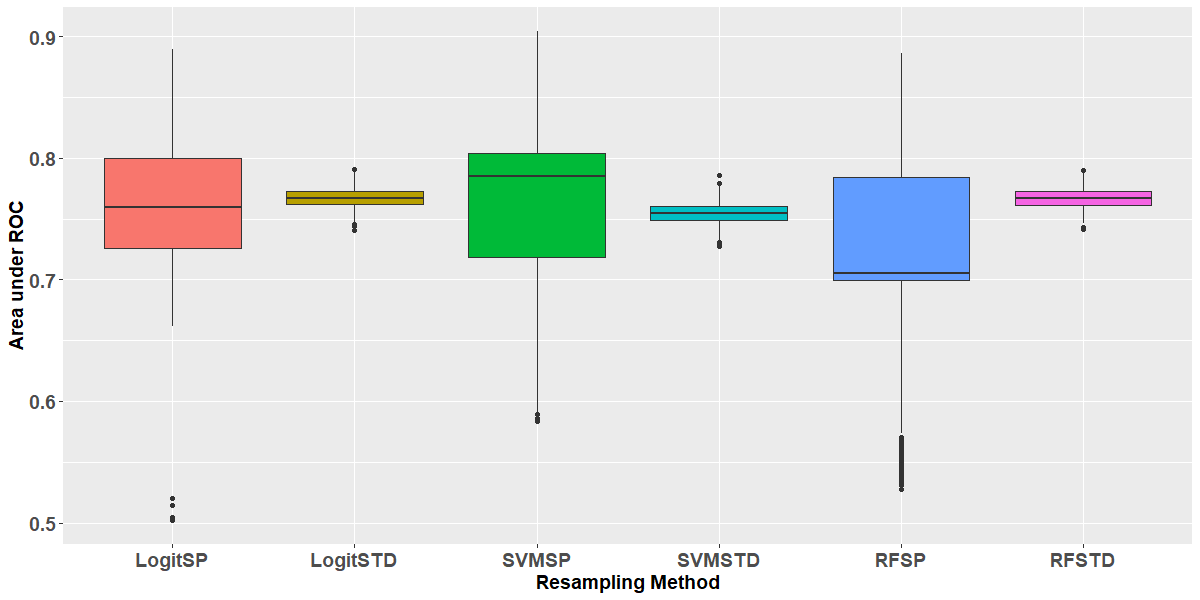
\includegraphics[width = 15cm, height = 7.5cm]{Figures/resamplingcomparison.png}
    \caption{Predictive Performance Vergleich der Modelle. ``SP'' entspricht repeated spatial CV; ``STD'' entspricht repeated standard CV}
    \label{performanceviz}
\end{figure}

Wie erwartet bewirkte die räumlich zusammenhängende CV eine Korrektur der mittleren Prognoseperformance der Modelle für logistisches- und Random Forest Modell nach unten. Überraschend ist der mittlere Performancegain für den SVM Klassifikator. Zur Erklärung dieses Phänomens wären weitere Untersuchungen nötig. Die Variation aller spatial Schätzer steigerte sich drastisch verglichen mit den Schätzern aus den standard CV Verfahren. Dies könnte ein Indiz dafür sein, dass ein sehr großes Forschungsareal wie Gesamtbayern nicht optimal für diese Resamplingmethode ist. Eventuell könnte es sinnvoll sein, das Forschungsareal vorab in kleinere Areale zu unterteilen (Ähnlich der nested CV) und dann innerhalb dieser kleineren Areale zu modellieren. Auch an Abbildung \ref{resamplingviz} wird erkennbar, dass sich bei repeated spatial CV Trainingsdatensätze ergeben können in denen ein Großteil der Sites, enthalten ist. Die allgemeine räumliche Verteilung der Sites scheint in Kombination mit dem gewählten Areal eventuell problematisch für dieses Verfahren zu sein. 
\newpage

\section{Interpretation und Probleme}
\label{section:5}
Die angewendeten Methoden schienen für das Erstellen von Prognosekarten ideal, allerdings lassen die starke Streuung der spatial Vorhersageschätzer vermuten, dass das Forschungsareal zu groß gewählt sein könnte. Die predictive Maps selbst sollten  aus ökologischer bzw. archäologischer Sicht weniger als ``Chance'' einen Fund im entsprechenden Rasterpixel zu machen, sondern mehr als Index für die Habitateignung der Rasterzellen für Menschen aus der Eisenzeit interpretiert werden. Des Weiteren ist das kontrastreiche Ergebnis des Random Forest Modells unter Umständen zu bevorzugen, da dieses die konservativsten Vorhersagen macht. Aus archäologischer Sicht ist dies durchaus erwünscht, schließlich bringen Ausgrabungen große Kosten mit sich und sollten auf stichhaltigen Beweisen basieren. Insgesamt sind die Ergebniskarten mit Vorsicht zu genießen; die Auflösung von der benutzten Rasterdaten ist zu gering um wirklich sinnvolle Prognosen aufzustellen. Es bieten sich Folgeuntersuchungen an, die kleinere Teilareale Bayerns mit höherauflösenden Rasterdaten analysieren könnten. Abgesehen davon sollte das in Kapitel 2 angesprochene Problem zum Finden eines idealen Bufferradius zum Samplen von pseudo-nonpräsenz Punkten tiefergehend untersucht werden.
\newpage

\section{Ausblick}
\label{section:Ausblick}
Die präsentierten Verfahren zur Untersuchung räumlicher Daten zeigten sich als angemessen für die Erstellung von predictive Maps. Aus performancetechnischer Sicht konnte der SVM Ansatz am stärksten überzeugen, allerdings sind die erhaltenen Karten mit Vorsicht zu interpretieren. \\ In erster Linie ist die Auflösung der verwendeten Rasterdaten zu gering für akurate Prognosen, aber auch die räumliche Konstantheit der geschätzten Koeffizienten des Logit-Modells und das Finden eines optimalen Bufferradius zum Sampling von non-presence Punkten sind unter Umständen problematisch. Abgesehen davon stellte sich heraus, dass beide der zum Tuning der Modelle und Einschätzen der predictive performance dieser, angewendeten Resamplingverfahren nicht ideal sind, um für räumlich korrelierte Daten in einem großen Gebiet wie Bayern sinnvolle Ergebnisse zu produzieren.  
Um die Problematik der Bestimmung eines "optimalen" Bufferradius zu umgehen bieten sich Maximum-Entropy Verfahren \cite{phillips2006maximum} oder der Punktprozessanalyse  an, welche zur Habitatmodellierung ohne Nonpräsenzdaten herangezogen werden können.\\
Natürlich sollte auch nicht unerwähnt bleiben, dass der Rasterstack aus Daten der Moderne zusammengefügt wurde, welche im Allgemeinen nicht repräsentativ für die tatsächliche Habitatsituation in der Eisenzeit sind. (Main-Donau Kanal im Gewässernetz etc.) \\
Darüber hinaus ließe sich mittels Gaußprozess-Regression \cite{gaussprozess} oder ähnlichen Verfahren zur Interpolation diskreter, räumlich korrelierter Messdaten das manuelle Zusammentragen eines Referenzdatensatzes zur Erzeugung von Nonpräsenzdaten vermeiden um direkt auf Basis der von Fender bereitgestellten Daten predictive Maps zu generieren. \\
Abschließend war die Bearbeitung georeferenzierter Daten mit Techniken aus dem maschinellen Lernen ein ausgesprochen interessantes Problem. 
\newpage

\sloppy
\printbibliography

\newpage
\listoffigures
\newpage
\listoftables

\end{document}